\scanpage{101}
\deleted{\unsure{Pro-schématiques} \unsure{sur} \unsure{k}}

\diagram{\begin{tikzcd}[ampersand replacement=\&,column sep=large]
(\text{Ens. }\unsure{\text{schématiques}}\text{ }\unsure{\text{sur}}\ k)
\arrow[r,"\text{pl. fidèle}"'] \& \underline{\operatorname{Hom}}((\text{Ens }\unsure{\text{schém.}}/k),(\text{Ens}))
\end{tikzcd}}

\diagram{\begin{tikzcd}[ampersand replacement=\&]
\& X \& \\
S \arrow[ur,dashed,"\unsure{\exists}"] \& S'\arrow[l]\arrow[u] \& S''\arrow[l,shift left]\arrow[l,shift right]
\end{tikzcd}}

\uuline{application surjective}\hfill\uline{\unsure{morphisme} fid. plat}

\uline{Tout épimorphisme est un morphisme de descente}

\[
\left\{\begin{array}{l}
\left[\begin{array}{ll}
1)&\text{Existence de }\varprojlim\text{ finies}\\
2)&\text{Existence du }\unsure{\text{quot}}\text{ par un graphe d'équivalence}
\end{array}\right.\\[4pt]
\left[\begin{array}{ll}
3)&\deleted{\text{Tout}}\ \text{épim est effectif}\\
4)&\text{Tout épim est universel}
\end{array}\right.
\end{array}\right.
\]
\margin{[\unsure{donc ça marche} pour \unsure{principes} d'\unsure{équivalence}\ldots]}

\deleted{5) Tout morphisme se factorise par un \unsure{produit} \unsure{des} [\unsure{épim}, \unsure{monom}]}

\diagram{\begin{tikzcd}[ampersand replacement=\&,column sep=small,execute at end picture={\draw (0.4,0.5) ellipse (2.3cm and 0.9cm);\draw (-2.9,0.25)--(-1.55,0.25);}]
\deleted{\unsure{E}}\arrow[r] \& X\times_Y X\arrow[r,shift left]\arrow[r,shift right] \& X\arrow[r]\arrow[dr] \&Y\\
\&\&\&X'\arrow[u,hook,"\unsure{\text{mon}}"']
\end{tikzcd}}

\[
\left\{\begin{array}{l}
\left[\begin{array}{ll}
1')&\text{Existence de }\varinjlim\text{ finies}\\
2')&\text{Existence du }\unsure{\text{coquotient}}\text{ par un cographe d'équivalence}
\end{array}\right.\\[4pt]
\left[\begin{array}{ll}
3')&\text{Tout mon est effectif}\\
4')&\unsure{\text{Co-changement}}\text{ de base }\unsure{\text{dans un}|\text{d’un}}\text{ monomorphisme}
\end{array}\right.
\end{array}\right.
\]
\margin{?}
\figure{\begin{tikzpicture}\draw (0,4.4) .. controls (.2,3.2) and (1.7,2.8) .. (2.8,2.5) .. controls (3.3,2.1) and (2.7,1.3) .. (2.8,0);\end{tikzpicture}}

\uline{Axiome géométrique}\qquad
$X\times\coprod Y_i\simeq\coprod_i X\times Y_i$

[\unsure{ou aussi}: \unsure{chgt} de base commute aux sommes,
-- donc aux $\varinjlim$ finies ???]

\diagram{\begin{tikzcd}[ampersand replacement=\&]R\arrow[r]\&S\end{tikzcd}}
\figure{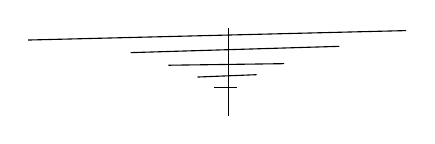
\begin{tikzpicture}[x=1cm,y=1cm]
\draw (-2.4,0)--(2.4,0.12);
\draw (-1.1,-0.16)--(1.55,-0.08);
\draw (-0.62,-0.32)--(0.85,-0.30);
\draw (-0.25,-0.47)--(0.50,-0.44);
\draw (-0.04,-0.60)--(0.25,-0.60);
\draw (0.14,0.15)--(0.14,-0.96);
\end{tikzpicture}}
\margin{100}
